% MATH 201 Lab notes (c) by Carlos Contreras And Philippe Gaudreau
% MATH 201 Lab notes is licensed under a 
% Creative Commons Attribution 4.0 International license.
% CC BY 4.0

% You should have received a copy of the license along with this
% work. If not, see <http://creativecommons.org/licenses/by/4.0/>.

\documentclass[11pt]{article}
% MATH 201 Lab notes (c) by Carlos Contreras And Philippe Gaudreau
% MATH 201 Lab notes is licensed under a 
% Creative Commons Attribution 4.0 International license.
% CC BY 4.0

% You should have received a copy of the license along with this
% work. If not, see <http://creativecommons.org/licenses/by/4.0/>.

%% libraries
\usepackage[utf8x]{inputenc}
\usepackage{xcolor}
\usepackage[left=1.5cm,right=1.5cm,top=2.0cm,bottom=1.5cm,headheight=110pt]{geometry}
\usepackage{amsmath}
\usepackage{amssymb}
\usepackage{graphicx}
\usepackage{xifthen}
\usepackage{sverb}
\usepackage{fancyhdr}
\usepackage{mdframed}
\usepackage{textcomp}

%%%%%%%%%%%%%%%%%%%%%%%%%%%%%%%%%%%%%%%%%%%%%%%%%%%%%%%%%%%%%%%%%%%%%%%
% PDF compiling
\usepackage{ifpdf}
\ifpdf %
        \DeclareGraphicsExtensions{.pdf}%
\else %
        \DeclareGraphicsExtensions{.eps,.ps}%
\fi

%%%%%%%%%%%%%%%%%%%%%%%%%%%%%%%%%%%%%%%%%%%%%%%%%%%%%%%%%%%%%%%%%%%%%%%
% Figures path
\graphicspath{{figures/}}

%%%%%%%%%%%%%%%%%%%%%%%%%%%%%%%%%%%%%%%%%%%%%%%%%%%%%%%%%%%%%%%%%%%%%%%
% Problem counter
\newcounter{Problem}
\setcounter{Problem}{0}

%%%%%%%%%%%%%%%%%%%%%%%%%%%%%%%%%%%%%%%%%%%%%%%%%%%%%%%%%%%%%%%%%%%%%%%
% Definitions
\def\LabSolutions{\clearpage \newpage \begin{center} {\Large \it Solutions} \end{center} \setcounter{Problem}{0}}
\def\QuizSolutions{\newpage \begin{center} {\Large \it Solutions} \end{center} \setcounter{Problem}{0}}
\def\degree{\textdegree}
\def\grade#1{\begin{flushright} {\small [#1]}\\ \end{flushright} \vspace{-10pt}}
\def\codecolor{red!50!black}
\def\code#1{\textcolor{\codecolor}{\tt #1}}
\def\examname#1{%
                \ifnum\value{page}>1%
                    \newpage%
                \else%
                    \vspace*{5pt}%
                \fi%
                \large \textbf{#1} \setcounter{Problem}{0}\vspace{10pt}}
\def\topic#1{\par\needspace{2\baselineskip} \noindent \textsl{\footnotesize #1}}

 
%%%%%%%%%%%%%%%%%%%%%%%%%%%%%%%%%%%%%%%%%%%%%%%%%%%%%%%%%%%%%%%%%%%%%%%
% Environments
\newenvironment{problem}%
     {\stepcounter{Problem}%
      \begin{list}{\textbf{\arabic{Problem}}.~}{}%
      \item}%
     {\end{list}\vspace*{5pt}}

\newenvironment{solution}%
     {\indent \textit{Solution} \newline}%
     {\begin{flushright}$\blacksquare$\end{flushright}}

\newenvironment{preamble}%
     {\vspace*{1em}\begin{mdframed}[leftmargin=1cm,rightmargin=1cm]}%
     {\end{mdframed}\vspace*{1em}}

\newenvironment{multchoice}%
     {\begin{enumerate} \addtolength{\leftskip}{2em} \renewcommand{\labelenumi}{(\alph{enumi})}}
     {\end{enumerate}}

\newenvironment{formulaitem}%
     {\setlength{\leftmargini}{1.5em}\begin{itemize}%
      \setlength\itemindent{-\itemindent}%
      \renewcommand{\labelitemi}{$\rightarrow$}}%
     {\end{itemize}}


%%%%%%%%%%%%%%%%%%%%%%%%%%%%%%%%%%%%%%%%%%%%%%%%%%%%%%%%%%%%%%%%%%%%%%%
% New theorems
\newtheorem{theorem}{Theorem}


\makeatletter

%%%%%%%%%%%%%%%%%%%%%%%%%%%%%%%%%%%%%%%%%%%%%%%%%%%%%%%%%%%%%%%%%%%%%%%
%% New commands
\newcommand*{\course}[1]{\gdef\@course{#1}}
\newcommand*{\coursecode}[1]{\gdef\@coursecode{#1}}
\newcommand*{\term}[1]{\gdef\@term{#1}}
\newcommand*{\instructor}[1]{\gdef\@instructor{#1}}
\newcommand*{\lqnumber}[1]{\gdef\@lqnumber{#1}}
\newcommand*{\labtitle}[1]{\gdef\@labtitle{#1}}
\newcommand*{\quizversion}[1]{\gdef\@quizversion{#1}}
\newcommand*{\probleminfo}[1]{\noindent \textsl{\footnotesize #1}}

% Title header for labs
\newcommand\makelabtitle{%
  \begin{flushleft}%
  {\scshape \@coursecode~\@course~-- University of Alberta}\\%
  {\scshape \@term~-- Labs -- \@instructor}\\%
  {\scshape Authors: Carlos Contreras and Philippe Gaudreau}%
  \end{flushleft}%
  \begin{center}%
  {\Large \bf \@lqnumber:~\@labtitle}%
  \end{center}%
  \thispagestyle{empty}%
  \global\let\@course\@empty%
  \global\let\@labtitle\@empty%
}

% Title header for quizzes
\newcommand\makequiztitle{%
  \begin{flushleft}%
  {\scshape \@coursecode~\@course~-- University of Alberta}\\%
  {\scshape \@term~-- Labs -- \@instructor}\\%
  \end{flushleft}%
  \begin{center}%
  {\Large \bf \@lqnumber} \marginpar{\tiny\tt [\@quizversion]}%
  \end{center}%
  \thispagestyle{empty}%
  \global\let\@course\@empty%
  \global\let\@quizversion\@empty%
}

%%%%%%%%%%%%%%%%%%%%%%%%%%%%%%%%%%%%%%%%%%%%%%%%%%%%%%%%%%%%%%%%%%%%%%%
% Fancy header package
\fancyhead[L]{\small {\scshape \@coursecode~-- \@lqnumber~-- \@term~-- \@instructor}}
\pagestyle{fancy}

\makeatother


\usepackage{hyperref}
\usepackage{cancel}


\begin{document}

\course{Differential Equations}
\coursecode{MATH 201}
\term{Winter 2018}
\instructor{Carlos Contreras}
\lqnumber{Lab 2}
\labtitle{Second-order homogeneous differential equations}
\makelabtitle




% real roots
\begin{problem}
Find a general solution to the given differential equation
\begin{equation*}
3y'' + 11y' - 7 y =0
\end{equation*}
\end{problem}


% real roots IVP
\begin{problem}
Find a general solution to the given differential equation
\begin{equation*}
y'' +y' -6y =0, \quad y(0)=2, \quad y'(0)=-\frac{17}{2}
\end{equation*}
\end{problem}



% real roots IVP
\begin{problem}
Find a solution to the given initial value differential equation
\begin{equation*}
z^{\prime \prime} -2 z^{\prime} -2z=0, \quad z(0) =0, \quad z^{\prime}(0) = 3
\end{equation*}
\end{problem}



% complex roots
\begin{problem}
Find a general solution to the given differential equation
\begin{equation*}
y^{\prime \prime} -10 y^{\prime} +26 y =0.
\end{equation*}
\end{problem}


% complex roots IVP
\begin{problem}
Find a solution to the given inital value differential equation
\begin{equation*}
y^{\prime \prime} -2 y^{\prime} +2 y =0, \quad y(\pi)=e^{\pi}, \quad y'(\pi)=0.
\end{equation*}
\end{problem}


% repeated roots
\begin{problem}
Find a general solution to the given differential equation
\begin{equation*}
4 w^{\prime \prime} + 20 w^{\prime} +25 w =0.
\end{equation*}
\end{problem}



% real, repeated and complex roots
\begin{problem}
Find a solution to the given initial value differential equation for $b=5, 4$ and $2$
\begin{equation*}
y^{\prime \prime} + b y^{\prime} + 4 y =0, \quad, y(0)=1, \quad y'(0)=0,
\end{equation*}
sketch the three solutions for $t>0$ and see how the solutions change with $b$.
\end{problem}




%%%%%%%%%%%%%%%%%%%%%%%%%%%%%%%%%%%%%%%%%%%%%%%%%%%%%%%%%%%%%%%%%%%%%%%%%%%%%%%%%%%%%%%%%%%%%%%%%%%



\LabSolutions


All problems from: Nagel, Saff \& Sneider, \textit{Fundamentals of Differential Equations}, Eight Edition, Adisson--Wesley.


\begin{preamble}
\begin{formulaitem}
     \item For the \textbf{second-order equation homogeneous with constant coefficients}
     \[ay''+by'+cy=0\]
     there are three posible solutions depending on the roots $r_{1}$ and $r_{2}$ of the auxiliary equation 
     \[ar^{2}+br+c=0.\]
     The three cases are:
     \begin{align*}
     \text{Case 1:} \quad y(t)&=C_{1}e^{r_{1}t}+C_{2}e^{r_{2}t}, \quad \text{if}\quad r_{1}\neq r_{2}, \\
     \text{Case 2:} \quad y(t)&=C_{1}e^{r_{1}t}+C_{2}te^{r_{1}t}, \quad \text{if}\quad r_{1}= r_{2}, \\
     \text{Case 3:} \quad y(t)&=C_{1}e^{\alpha t}\cos(\beta t )+C_{2}e^{\alpha t}\sin(\beta t ), \quad \text{if}\quad r_{1}, r_{2} = \alpha \pm i \beta.
     \end{align*}
\end{formulaitem}

\end{preamble}



% real roots
\begin{problem}
Find a general solution to the given differential equation
\begin{equation*}
3y'' + 11y' - 7 y =0
\end{equation*}
\end{problem}
\begin{solution}
The auxiliary equation for this ODE is the following
\begin{equation*}
3r^2 +11r -7 =0 \Rightarrow r = \frac{-11\pm \sqrt{205}}{6}.
\end{equation*}
The general solution is then given by:
\begin{equation*}
\boxed{ z(t) = C_{1} e^{(-11 + \sqrt{205}) t/6} + C_{2} e^{-(11 + \sqrt{205})t/6}}.
\end{equation*}
\end{solution}



% real roots
\begin{problem}
Find a general solution to the given differential equation
\begin{equation*}
y'' +y' -6y =0, \quad y(0)=2, y'(0)=-\frac{17}{2}
\end{equation*}
\end{problem}
\begin{solution}
The auxiliary equation for this ODE is the following
\begin{equation*}
r^2 +r -6 =0 \Rightarrow r = 2, \,\, \text{and} \,\,r = -3.
\end{equation*}
The general solution is then given by:
\begin{equation*}
y(t) = C_{1} e^{2 t} + C_{2} e^{-3 t}.
\end{equation*}
Taking the derivative, we find:
\begin{equation*}
y^{\prime}(t) = 2C_{1}  e^{2 t} - 3C_{2} e^{ -3 t}.
\end{equation*}
Setting $t=0$ in both equation, we obtain:
\begin{eqnarray*}
2 &=& C_{1} + C_{2} ,\\
-\frac{17}{2} &=& 2C_{1} - 3C_{2} .
\end{eqnarray*}
Solving this system, we obtain: $C_{1} = -\frac{1}{2}$ and $C_{2} = \frac{5}{2}$.
Hence, the solution to this IVP is
\begin{equation*}
\boxed{ y(t) = -\dfrac{1}{2} e^{2 t} + \dfrac{5}{2} e^{-3 t}}.
\end{equation*}
\end{solution}


% real roots IVP
\begin{problem}
Find a solution to the given initial value differential equation
\begin{equation*}
z^{\prime \prime} -2 z^{\prime} -2z=0, \quad z(0) =0, \quad z^{\prime}(0) = 3
\end{equation*}
\end{problem}
\begin{solution}
The auxiliary equation for this ODE is the following
\begin{equation*}
r^2 -2r -2 =0 \Rightarrow r = 1 \pm \sqrt{3}
\end{equation*}
The general solution is then given by:
\begin{equation*}
z(t) = C_{1} e^{(1 + \sqrt{3}) t} + C_{2} e^{(1 - \sqrt{3})t}
\end{equation*}
Taking the derivative, we find:
\begin{equation*}
z^{\prime}(t) = C_{1}(1 + \sqrt{3}) e^{(1 + \sqrt{3}) t} + C_{2}(1 - \sqrt{3}) e^{(1 - \sqrt{3})t}
\end{equation*}
Setting $t=0$ in both equation, we obtain:
\begin{eqnarray*}
0 &=& C_{1} + C_{2} \\
3 &=& C_{1}(1 + \sqrt{3}) + C_{2}(1 - \sqrt{3})
\end{eqnarray*}
Solving this system, we obtain: $C_{1} = \dfrac{\sqrt{3}}{2}$ and $C_{2} = -\dfrac{\sqrt{3}}{2}$.
Hence the solution to this IVP is
\begin{equation*}
\boxed{ z(t) = \dfrac{\sqrt{3}}{2} e^{(1 + \sqrt{3}) t} - \dfrac{\sqrt{3}}{2} e^{(1 - \sqrt{3})t}}.
\end{equation*}
\end{solution}


% complex roots
\begin{problem}
Find a general solution to the given differential equation
\begin{equation*}
y^{\prime \prime} -10 y^{\prime} +26 y =0
\end{equation*}
\end{problem}
\begin{solution}
The auxiliary equation for this ODE is the following
\begin{equation*}
r^2 -10r +26 =0 \Rightarrow r = 5 \pm i
\end{equation*}
The solution is then given by:
\begin{equation*}
\boxed{ y(t) = C_{1} e^{5 t} \cos(t) + C_{2} e^{5t} \sin(t)}.
\end{equation*}
\end{solution}


% complex roots
\begin{problem}
Find a solution to the given inital value differential equation
\begin{equation*}
y^{\prime \prime} -2 y^{\prime} +2 y =0, \quad y(\pi)=e^{\pi}, \quad  y'(\pi)=0
\end{equation*}
\end{problem}
\begin{solution}
The auxiliary equation for this ODE is the following
\begin{equation*}
r^2 -2r +2 =0 \Rightarrow r = 1 \pm i.
\end{equation*}
The general solution is then given by:
\begin{equation*}
y(t) = C_{1} e^{t} \cos(t) + C_{2} e^{t} \sin(t).
\end{equation*}
Taking the derivative, we find:
\begin{equation*}
y^{\prime}(t) = C_{1} e^{t} \cos(t) - C_{1} e^{t} \sin(t) + C_{2} e^{t} \sin(t) + C_{2} e^{t} \cos(t).
\end{equation*}
Setting $t=\pi$ in both equation, we obtain:
\begin{eqnarray*}
e^{\pi} &=& C_{1} e^{\pi}\cancelto{\scriptstyle -1}{\cos{\pi}} \quad+ C_{2} e^{\pi}\cancelto{\scriptstyle 0}{\sin{\pi}} ,\\
0 &=& C_{1} e^{\pi}\cancelto{\scriptstyle -1}{\cos{\pi}} \quad- C_{1} e^{\pi}\cancelto{\scriptstyle 0}{\sin{\pi}} \quad + C_{2} e^{\pi}\cancelto{\scriptstyle 0}{\sin{\pi}} \quad + C_{2} e^{\pi}\cancelto{\scriptstyle -1}{\cos{\pi}}.
\end{eqnarray*}
Solving this system, we obtain: $C_{1} = -1$ and $C_{2} = 1$.
Hence, the solution to this IVP is
\begin{equation*}
\boxed{ y(t) = -e^{t}\cos(t) + e^{t}\sin(t) }.
\end{equation*}
\end{solution}


% repeated roots
\begin{problem}
Find a general solution to the given differential equation
\begin{equation*}
4 w^{\prime \prime} + 20 w^{\prime} +25 w =0
\end{equation*}
\end{problem}
\begin{solution}
The auxiliary equation for this ODE is the following
\begin{equation*}
4r^2 +20r +25 =0 \Rightarrow r = -\frac{5}{2}
\end{equation*}
The solution is then given by:
\begin{equation*}
\boxed{ w(t) = C_{1} e^{-\frac{5}{2} t} + C_{2} t e^{-\frac{5}{2}t}}.
\end{equation*}
\end{solution}





% real, repeated and complex roots
\begin{problem}
Find a solution to the given initial value differential equation for $b=5, 4$ and $2$
\begin{equation}
\label{equ:prob07}
y^{\prime \prime} + b y^{\prime} + 4 y =0, \quad, y(0)=1, \quad y'(0)=0,
\end{equation}
sketch the three solutions for $t>0$ and see how the solutions change with $b$.
\end{problem}
\begin{solution}
The auxiliary equation for this ODE is the following
\begin{equation*}
r^2 + b r + 4 =0 \Rightarrow r = \frac{-b\pm \sqrt{b^{2}-16}}{2} =\frac{-b\pm \sqrt{\Delta}}{2},
\end{equation*}
and we have three options depending on the sign of $\Delta$
\begin{equation*}
\begin{split}
     \Delta_{5}&=25-16 =9 >0 \\
     \Delta_{4}&=16-16 = 0 \\
     \Delta_{2}&=4-16 = -12 <0 
\end{split}
\end{equation*}
These values where chosen so we have the three posible options: distinct real roots, repeated real root, and complex roots.\\
\textbf{For $\bf b=5$}. The roots are $r=-1$ and $r=-4$ (distinct real roots case). 
The general solution and its derivative are given by
\begin{equation*}
\begin{split}
y(t) &= C_{1} e^{-t}  + C_{2} e^{-4t} \\
y'(t) &= - C_{1} e^{-t}  -4 C_{2} e^{-4t}
\end{split}
\end{equation*}
Using the initial conditions we obtain
\begin{eqnarray*}
1 &=& C_{1} + C_{2},\\
0 &=& -C_{1} -4 C_{2}.
\end{eqnarray*}
Solving this system, we obtain $C_{1} = \frac{4}{3}$ and $C_{2} = -\frac{1}{3}$.
Hence, the solution to this IVP is
\begin{equation*}
\boxed{ y(t) = \frac{4}{3}e^{-t} - \frac{1}{3}e^{-4t}}.
\end{equation*}
\textbf{For $\bf b=4$}. The roots is $r=-2$ (repeated real root case).
The general solution and its derivative are given by
\begin{equation*}
\begin{split}
y(t) &= C_{1} e^{-2t}  + C_{2} te^{-2t} \\
y'(t) &= -2 C_{1} e^{-t} + C_{2}e^{-2t} -2 C_{2} t e^{-2t}
\end{split}
\end{equation*}
Using the initial conditions we obtain
\begin{eqnarray*}
1 &=& C_{1},\\
0 &=& -2C_{1} + C_{2}.
\end{eqnarray*}
Solving this system, we obtain $C_{1} = 1$ and $C_{2} = 2$.
Hence, the solution to this IVP is
\begin{equation*}
\boxed{ y(t) = e^{-2t} +2 t e^{-2t}}.
\end{equation*}
\textbf{For $\bf b=2$}. The roots is $r=-1\pm \sqrt{3}$ (complex roots case).
The general solution and its derivative are given by
\begin{equation*}
\begin{split}
y(t) &= C_{1} e^{-t}\cos(\sqrt{3}t)  + C_{2} e^{-t}\sin(\sqrt{3}t) \\
y'(t) &= - C_{1} e^{-t}\cos(\sqrt{3}t) - \sqrt{3}C_{1} e^{-t}\sin(\sqrt{3}t) - C_{2}e^{-t}\sin(\sqrt{3}t) + \sqrt{3}C_{2}e^{-t}\cos(\sqrt{3}t)
\end{split}
\end{equation*}
Using the initial conditions we obtain
\begin{eqnarray*}
1 &=& C_{1} \cos 0 + C_{2}\sin 0,\\
0 &=& -C_{1} \cos 0 - \sqrt{3}C_{1} \sin 0 - C_{2} \sin 0 + \sqrt{3} C_{2}\cos 0.
\end{eqnarray*}
Solving this system, we obtain $C_{1} = 1$ and $C_{2} = \frac{\sqrt{3}}{3}$.
Hence, the solution to this IVP is
\begin{equation*}
\boxed{ y(t) = e^{-t}\cos(\sqrt{3}t) + \frac{\sqrt{3}}{3} e^{-t}\sin(\sqrt{3}t)}.
\end{equation*}
Decreasing $b$ from $5$ to $4$ the tail of the curve becomes heavier (see Figure \ref{fig:prob07}), and at $b=4$ the the roots crosses to the imaginary part and the solution oscilates. Note that each solution (particularly in the complex case) is bounded, e.g, by $\pm 2e^{-t}$.
\begin{figure}
\begin{center}
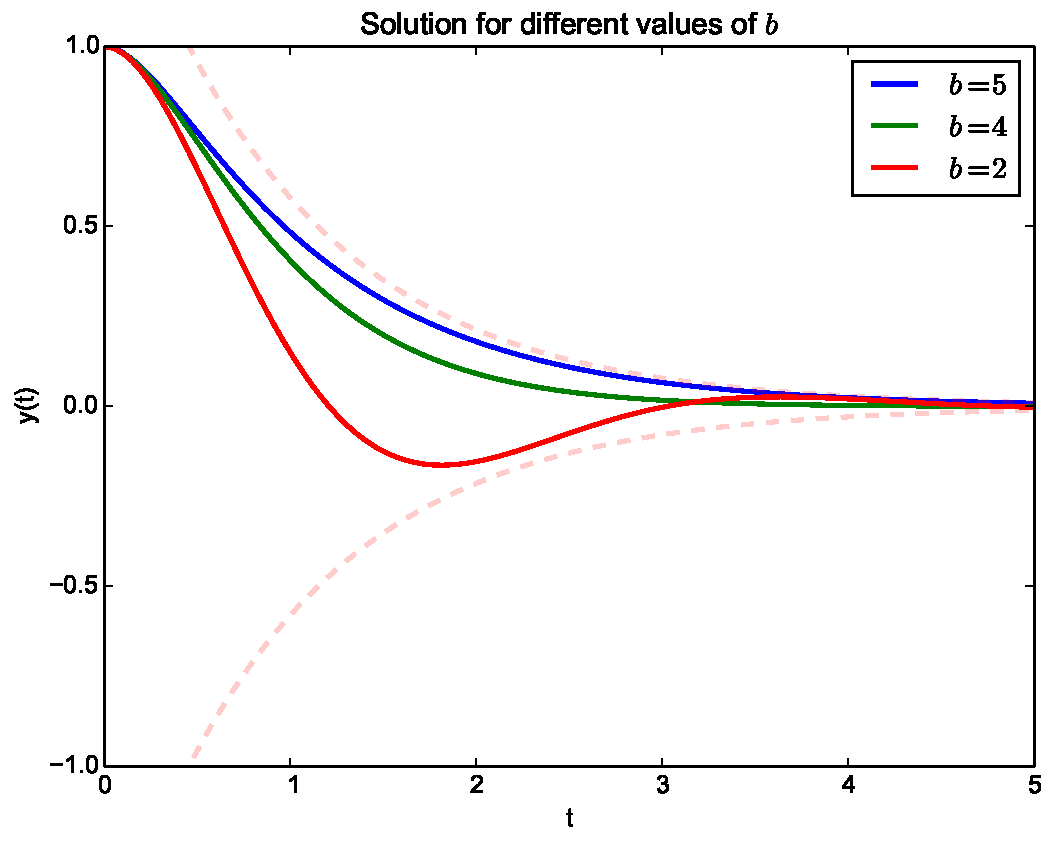
\includegraphics[width=0.5\linewidth]{figures/lab02prob07.pdf}
\caption{Solution to IVP \eqref{equ:prob07} for $b=5, 4$ and $2$.}
\label{fig:prob07}
\end{center}

\end{figure}

\end{solution}















\end{document}
